% !TEX encoding = UTF-8
% !TEX TS-program = pdflatex
% !TEX root = ../tesi.tex

%**************************************************************
\chapter{Strumenti e tecnologie}
\label{cap:strumenti}
%**************************************************************

%\intro{Breve introduzione al capitolo}\\

%**************************************************************
Per poter eseguire il confronto tra le prestazioni di database relazionali e NoSQL, è stato necessario preparare diversi strumenti utili a far funzionare i database stessi e al monitoraggio dei dati contenuti al loro interno.

%**************************************************************
\section{Docker}
Per poter effettuare test consistenti, evitare problemi di installazione e compartimentalizzare l'ambiente di lavoro, si è deciso di sfruttare Docker \cite{site:docker}\cite{site:dockerdocs} (logo in \autoref{fig:docker}). Questo software permette di virtualizzare l'esecuzione di altri applicativi in ambienti chiusi e controllati, facilitando determinati processi di sviluppo. L'utilizzo di Docker in questo progetto lo rende più maneggevole e lineare.\\

\noindent Per poter utilizzare Docker è necessario prima comprendere alcune parole chiave e ciò che esse rappresentano \cite{site:fireshipdocker}:
\begin{itemize}
    \item \textit{Dockerfile}
    \item \textit{Image}
    \item \textit{Container}
\end{itemize}
Il dockerfile racchiude una serie di istruzioni che servono a Docker per sapere come costruire un'immagine.\\
Questa, a sua volta, è uno snapshot del software che vogliamo utilizzare, comprese tutte le sue dipendenze, fino al sistema operativo. Questa immagine viene messa all'interno di un container per poter utilizzare il suddetto software.\\
Le immagini di molti software sono disponibili online e possono essere utilizzate come template da cui partire all'interno del dockerfile.\\
Una volta creata un'immagine, è possibile usarla in quanti container si desidera, e la si può mettere a disposizione di altri utenti perché possano utilizzare lo stesso ambiente su macchine diverse.\\
In questo senso, Docker è di fatto molto simile ad una \textit{Virtual Machine}, con la differenza (cruciale) che mentre all'interno di una \textit{VM} viene fatto girare un sistema operativo ``ospite'', ed ogni macchina virtuale ne utilizza uno a sè stante, i container di docker condividono lo stesso \textit{kernel}, il Docker Engine, rendendo questo sistema molto più leggero e veloce.\\
Docker permette quindi di creare più container che funzionano parallelamente e possono comunicare tra loro, rimanendo indipendentementi dagli altri container e dal sistema operativo in cui eseguiamo il Docker Engine.\\

\noindent Nel caso di questo progetto, Docker risulta utile innanzitutto per gestire il funzionamento dei due database (che saranno PostgreSQL e MongoDB), che verranno quindi inseriti in appositi container.\\
Per facilitare poi i processi di comunicazione con i database verranno utilizzati altri due container contenenti delle interfacce grafiche per la gestione dei dati (rispettivamente pgAdmin e mongo-express).

\begin{figure}[htbp]
\begin{center}
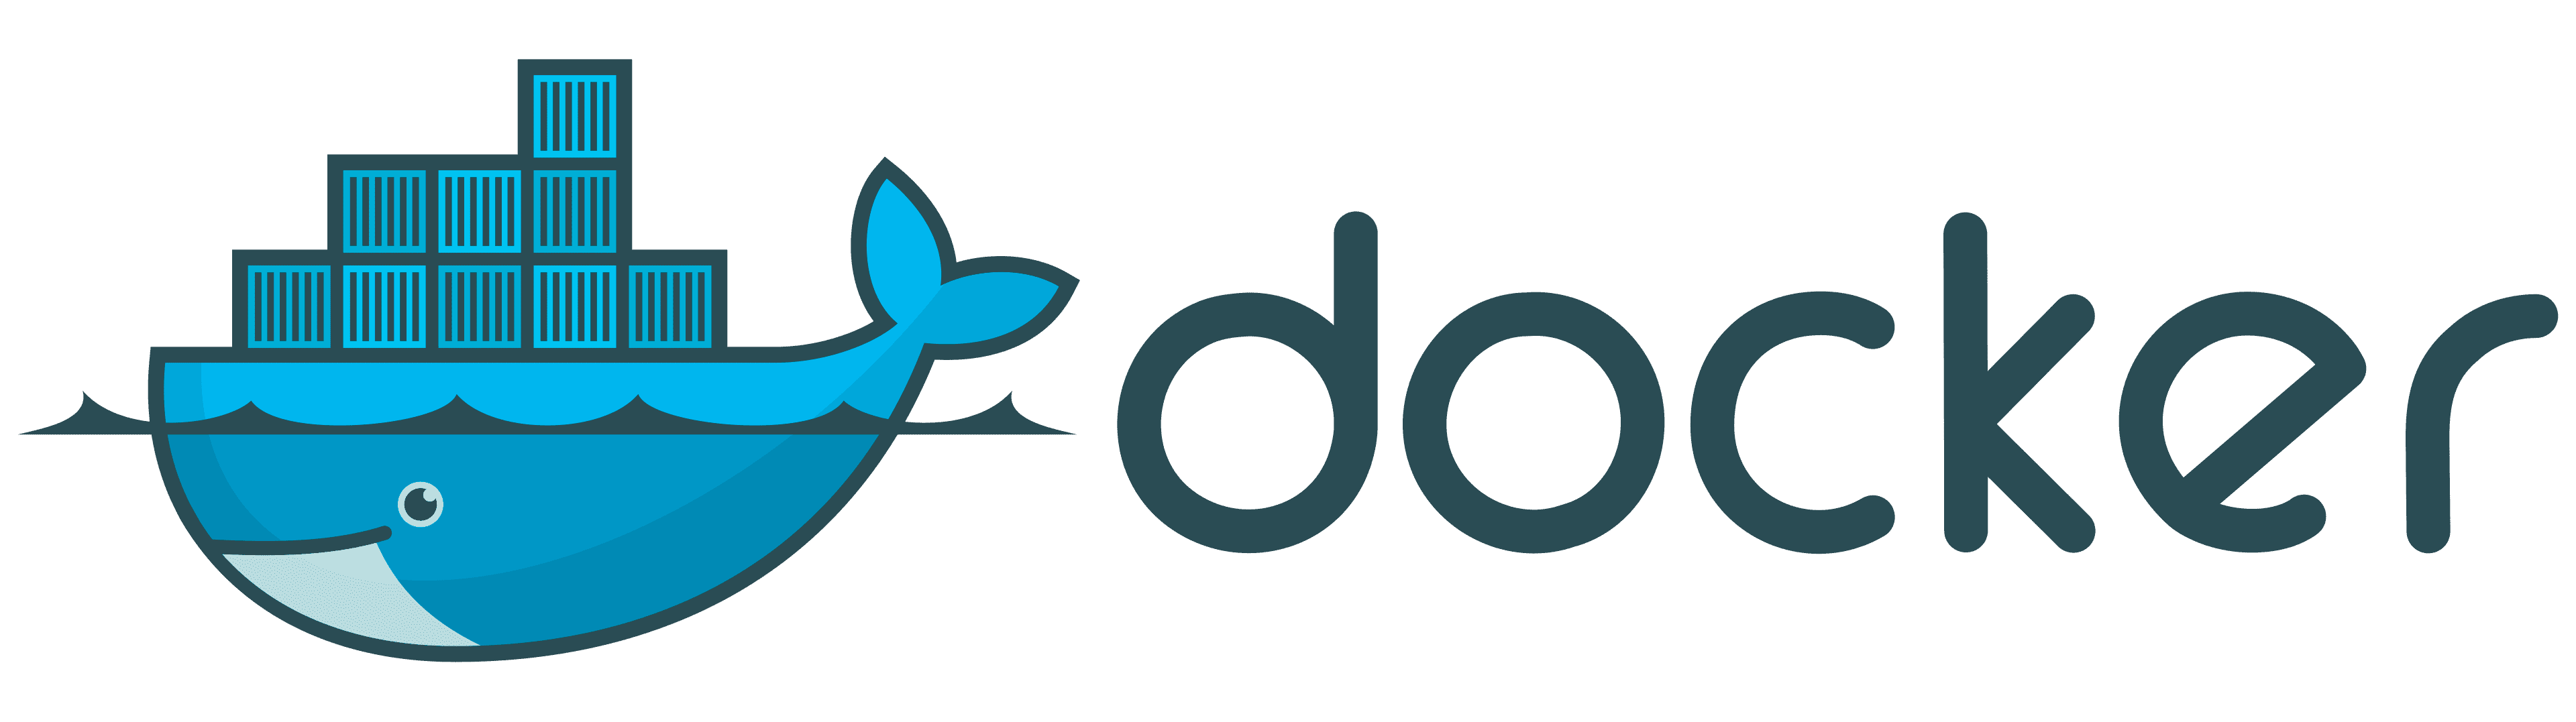
\includegraphics[height=6em]{immagini/tecnologies-logos/Docker-Logo.png}
\caption{Logo di Docker}
\label{fig:docker}
\end{center}
\end{figure}

%**************************************************************
\section{PostgreSQL e tecnologie annesse}
Dopo aver scelto Docker come ambiente in cui montare i database, alcune altre scelte legate alle tecnologie coinvolte in questa ricerca sono state prese di conseguenza.\\
Sebbene infatti sia possibile \textit{dockerizzare} moltissimi software, per gli scopi di questa tesi è risultato più sensato partire da immagini pre-esistenti ed affidabili, disponibili sulla piattaforma ufficiale del software (hub-docker).\\
Questo ha permesso di non investire troppo tempo nella preparazione degli strumenti e di concentrare le risorse disponibili nell'effettivo confronto tra database.\\

\noindent Per tutti questi motivi si è quindi scelto di usare PostgreSQL (logo in \autoref{fig:postgresql}) come database relazionale da portare a confronto con MongoDB.\\
PostreSQL è un database relazionale \textit{open source} molto robusto che si presta bene per rappresentare le prestazioni di un generico database di questa categoria \cite{site:postgres}. Esso è inoltre presente nell'hub di docker con un'immagine ufficiale, ed è quindi facile da far funzionare all'interno di un container a differenza di altri prodotti simili.\\
Sebbene PostgreSQL non sia utilizzato massivamente all'interno dell'azienda, risulta comunque molto simile alle sue controparti non open source, \textit{MSSQL} e \textit{Oracle Server}, che sono invece largamente usate all'interno di Ifin e sarebbero oggetto di una potenziale migrazione qualora i risultati di questa tesi si rivelassero convincenti.\\

\noindent Vale la pena di evidenziare che, a differenza delle tecnologie che ricadono sotto la sigla NoSQL, quelle legate ai database relazionali sono molto più simili tra loro, poichè condividono appunto il paradigma relazionale che sta alla base di tutte le variazioni esistenti proposte da aziende diverse in contesti diversi.\\
In questo senso, usare PostgreSQL non è una scelta incoerente con i motivi che hanno dato alla luce questo progetto.\\

\noindent Oltre al container utilizzato per il database di PostgreSQL, è necessario poter utilizzare uno strumento per effettuare operazioni su di esso.\\
Come spiegato in fase di analisi dei software proprietari di Ifin, questi sfruttano diversi framework e paradigmi per poter comunicare con i database ed operare su di essi le \gls{operazioni CRUD}\ped{G} (\textit{Create, Read, Update, Delete}) necessarie al funzionamento del software stesso. Considerato l'obiettivo di questa ricerca non avrebbe tuttavia senso investire tempo nel setup di un software dedicato a questi scopi.\\
Esistono infatti delle interfacce che ci permettono di interagire ``manualmente'' con i database senza fare uso di codice ed altre infrastrutture nel mezzo.\\
Per quanto riguarda PostgreSQL, la scelta è ricaduta su pgAdmin, un'interfaccia molto popolare e ben mantenuta, disponibile come immagine nella hub di docker per essere utilizzata all'interno di un container. È quindi sufficiente mettere in comunicazione i due container, uno per PostgreSQL e uno per pgAdmin, per avere a disposizione un ambiente completo in cui effettuare test su database relazionali.

\begin{figure}[htbp]
\begin{center}

\includegraphics[height=7em]{immagini/tecnologies-logos/postgresql-logo.png}
\caption{Logo di PostgreSQL}
\label{fig:postgresql}
\end{center}
\end{figure}

%**************************************************************
\section{MongoDB e tecnologie annesse}
Come già anticipato in \autoref{sec:fineindagine}, per mettere a confronto le potenzialità dei database NoSQL rispetto a quelli di tipo relazionale è stato scelto MongoDB (logo in \autoref{fig:mongodb}).\\
Anche in questo caso la scelta è stata guidata da più fattori che rendono MongoDB il candidato perfetto per questa ricerca.\\
Lo schema dinamico su cui esso si basa, assieme alla struttura dei dati che permette di immagazzinare, rappresentano fattori che potrebbero migliorare il modo in cui le informazioni vengono tutt'ora gestite ed archiviate da Ifin.\\
La popolarità di MongoDB determina inoltre un'abbondanza di guide e documentazione a cui fare riferimento per condurre un'analisi accurata delle sue potenzialità.\\
Infine, anche per questo database esiste un'immagine, mantenuta ufficialmente dal team di MongoDB, per poterlo utilizzare come container all'interno di Docker.\\

\noindent Per quanto riguarda l'interazione con il database e l'utilizzo di \gls{operazioni CRUD}\ped{G} al suo interno, sono stati utilizzati principalmente due strumenti.\\ 
In una fase iniziale in cui la necessità principale era quella di imparare e testare la sintassi delle operazioni sul database, un'interfaccia molto semplificata in grado di effettuare solo operazioni di inserimento e cancellazione dei dati è stata sufficiente. Si è quindi ricorso all'uso di mongo-express, un'interfaccia grafica molto basilare, il cui più grande pregio è quello di essere un software \textit{dockerizzabile}, eseguibile assieme al container dedicato a MongoDB e connesso ad esso seguendo le regole già apprese per connettere interfaccia e database di PostreSQL.\\
In un secondo momento, tuttavia, tale interfaccia non è più risultata sufficiente, dato il tipo di analisi che si è voluto condurre sui risultati delle query e sul loro tempo di esecuzione.\\
Si è quindi deciso di passare all'utilizzo di un'altra interfaccia grafica, MongoDB Compass, questa volta esterna all'ambiente di Docker, installata direttamente sulla postazione fornita da Ifin durante il tirocinio.\\
Compass è un software sviluppato direttamente dal team di MongoDB che mette a disposizione sia un'interfaccia grafica di facile utilizzo, sia un terminale da cui eseguire le operazioni più a basso livello, per poter utilizzare tutte le funzionalità che MongoDB ha da offrire.

\begin{figure}[htbp]
\begin{center}

\includegraphics[height=6em]{immagini/tecnologies-logos/MongoDB-Logo.png}
\caption{Logo di MongoDB}
\label{fig:mongodb}
\end{center}
\end{figure}

%**************************************************************
\section{Altri strumenti}
Oltre a quelli principali visti nelle sezioni precedenti, sono stati unilizzati altri strumenti di base per la stesura di appunti ed analisi, quali fogli di calcolo e documenti di testo, assieme ad altri software per la creazione dei dati di test da inserire nei database, che verrranno descritti in maggiore dettaglio nei capitoli successivi.\\
